\documentclass[aspectratio=169,11pt]{beamer}

\usepackage[utf8]{inputenc}
\usepackage[T5]{fontenc}
\usepackage[vietnamese,english]{babel}
\usepackage{amsmath}
\usepackage{booktabs}
\usepackage{graphicx}
\usepackage{tabularx}
\usepackage{xcolor}

\graphicspath{{assets/}}

\usetheme{Madrid}
\usecolortheme{default}
\setbeamertemplate{navigation symbols}{}

\definecolor{HustBlue}{HTML}{005BAA}
\definecolor{DeepBlue}{HTML}{003B73}
\definecolor{LightBlue}{HTML}{E8F3FF}
\definecolor{Accent}{HTML}{00A3E0}

\setbeamercolor{structure}{fg=HustBlue}
\setbeamercolor{palette primary}{fg=white,bg=DeepBlue}
\setbeamercolor{palette secondary}{fg=white,bg=HustBlue}
\setbeamercolor{palette tertiary}{fg=white,bg=DeepBlue}
\setbeamercolor{palette quaternary}{fg=white,bg=HustBlue}
\setbeamercolor{frametitle}{fg=white,bg=HustBlue}
\setbeamercolor{title}{fg=white,bg=DeepBlue}
\setbeamercolor{block title}{fg=white,bg=HustBlue}
\setbeamercolor{block body}{fg=black,bg=LightBlue}
\setbeamercolor{section in head/foot}{fg=white,bg=DeepBlue}
\setbeamercolor{subsection in head/foot}{fg=white,bg=HustBlue}
\setbeamercolor{author in head/foot}{fg=white,bg=DeepBlue}
\setbeamercolor{title in head/foot}{fg=white,bg=HustBlue}
\setbeamercolor{date in head/foot}{fg=white,bg=DeepBlue}

\setbeamertemplate{headline}{%
  \leavevmode%
  \hbox{%
    \begin{beamercolorbox}[wd=.48\paperwidth,ht=2.5ex,dp=1.05ex,leftskip=1em]{section in head/foot}%
      \usebeamerfont{section in head/foot}\insertsectionhead
    \end{beamercolorbox}%
    \begin{beamercolorbox}[wd=.52\paperwidth,ht=2.5ex,dp=1.05ex,rightskip=1em plus1fil]{subsection in head/foot}%
      \usebeamerfont{subsection in head/foot}\hfill\insertsubsectionhead
    \end{beamercolorbox}%
  }%
}

\setbeamertemplate{footline}{%
  \leavevmode%
  \hbox{%
    \begin{beamercolorbox}[wd=.30\paperwidth,ht=2.7ex,dp=1.15ex,leftskip=1em]{author in head/foot}%
      \usebeamerfont{author in head/foot}HUST -- IT4130E
    \end{beamercolorbox}%
    \begin{beamercolorbox}[wd=.50\paperwidth,ht=2.7ex,dp=1.15ex,center]{title in head/foot}%
      \usebeamerfont{title in head/foot}MPI Sinkhorn Solver
    \end{beamercolorbox}%
    \begin{beamercolorbox}[wd=.20\paperwidth,ht=2.7ex,dp=1.15ex,rightskip=1em plus1fil]{date in head/foot}%
      \usebeamerfont{date in head/foot}\hfill 2026 \quad \insertframenumber/\inserttotalframenumber
    \end{beamercolorbox}%
  }%
}

\setbeamertemplate{itemize item}{\color{HustBlue}$\blacktriangleright$}
\setbeamertemplate{itemize subitem}{\color{Accent}$\bullet$}

\newcolumntype{Y}{>{\raggedright\arraybackslash}X}
\newcolumntype{P}[1]{>{\raggedright\arraybackslash}p{#1}}

\title[MPI Sinkhorn Solver]{MPI Sinkhorn Optimal Transport Solver}
\subtitle{Row-wise Data Decomposition on a Physical VM Cluster}
\author{Nguyễn Tất Thanh \and Đặng Thịnh Tường Minh \and Nguyễn Ngọc Minh \and Kiều Sơn Tùng}
\institute{Hanoi University of Science and Technology\\School of Information and Communication Technology}
\date{2026}
\titlegraphic{
\includegraphics[height=1.15cm]{logo-soict-hust-1.png}}

\begin{document}

\begin{frame}
  \titlepage
\end{frame}

\section{Overview}
\subsection{Project requirements}

\begin{frame}{Project Goal and Deliverables}
\begin{columns}[T]
\begin{column}{0.52\linewidth}
\textbf{Assignment requirements}
\begin{itemize}
  \item C/C++ MPI implementation
  \item At least three physical machines
  \item Explain parallelism, decomposition, mapping, communication
  \item Validate correctness against sequential baseline
  \item Measure runtime, speedup, efficiency, and load balance
\end{itemize}
\end{column}
\begin{column}{0.44\linewidth}
\textbf{Delivered}
\begin{itemize}
  \item C++17 Sinkhorn solver
  \item Sequential and MPI modes
  \item Router/Ethernet and Wi-Fi cluster results
  \item JSON/CSV benchmark logs
  \item Dynamic scheduling extension
\end{itemize}
\end{column}
\end{columns}
\end{frame}

\section{Algorithm}
\subsection{Sinkhorn optimal transport}

\begin{frame}{Problem: Entropy-Regularized Optimal Transport}
\begin{columns}[T]
\begin{column}{0.52\linewidth}
Optimal transport finds a transport plan $P$ from source distribution $a$ to target distribution $b$.

\[
K_{ij} = \exp(-C_{ij}/\varepsilon)
\]
\[
u = a \oslash (Kv), \qquad v = b \oslash (K^Tu)
\]
\[
P = \mathrm{diag}(u)K\mathrm{diag}(v)
\]
\end{column}
\begin{column}{0.44\linewidth}
\textbf{Why this is parallelizable}
\begin{itemize}
  \item Dense $N \times N$ kernel matrix
  \item $O(N^2)$ work per iteration
  \item Row updates are independent
  \item Column update requires global reduction
\end{itemize}
\end{column}
\end{columns}
\end{frame}

\subsection{MPI row decomposition}

\begin{frame}{Parallel Algorithm}
\begin{columns}[T]
\begin{column}{0.50\linewidth}
\textbf{Data decomposition}
\begin{itemize}
  \item Split rows contiguously by MPI rank
  \item Rank $r$ owns $K_r = K[s_r:e_r, :]$
  \item Vector $v$ is replicated on all ranks
  \item Each rank updates local $u_i$
\end{itemize}
\end{column}
\begin{column}{0.46\linewidth}
\textbf{Communication}
\[
\mathrm{local\_col}_j =
\sum_{i=s_r}^{e_r-1} K_{ij}u_i
\]
\[
\mathrm{global\_col} =
\mathrm{MPI\_Allreduce}(\mathrm{local\_col})
\]
\begin{itemize}
  \item One length-$N$ Allreduce per iteration
  \item Main bottleneck at high process counts
\end{itemize}
\end{column}
\end{columns}
\end{frame}

\begin{frame}[fragile]{MPI Sinkhorn Pseudocode}
\small
\begin{verbatim}
Build local rows [s_r, e_r)
Build local dense kernel K_r
Initialize local u and replicated v

for iter = 1..max_iters:
    for each local row i:
        u[i] = a[i] / sum_j K_r[i,j] * v[j]

    local_col[:] = 0
    for each local row i:
        for each column j:
            local_col[j] += K_r[i,j] * u[i]

    global_col = MPI_Allreduce_sum(local_col)
    for each column j:
        v[j] = b[j] / global_col[j]
\end{verbatim}
\end{frame}

\section{Cluster}
\subsection{Hardware and network}

\begin{frame}{Cluster and Hardware}
\scriptsize
\begin{tabularx}{\linewidth}{P{1.35cm}P{2.15cm}P{0.9cm}P{1.05cm}P{1.55cm}P{1.9cm}Y}
\toprule
\textbf{Node} & \textbf{Physical CPU} & \textbf{C/T} & \textbf{VM CPU} & \textbf{VM RAM} & \textbf{GB6 score} & \textbf{Role} \\
\midrule
Master & Intel Core i5-9300H & 4/8 & 4 vCPU & 4 $\rightarrow$ 8 GB & 1291 SC / 3737 MC & Master for router and latest Wi-Fi runs \\
Worker 1 & Intel Core i5-9300H & 4/8 & 4 vCPU & 4 $\rightarrow$ 8 GB & 1291 SC / 3737 MC & Router/Wi-Fi worker \\
Worker 2 & AMD Ryzen 5 5600H & 6/12 & 4 vCPU & 3 $\rightarrow$ 6 GB & 1594 SC / 5716 MC & Router worker, stronger CPU but initially memory-limited \\
Worker 3 & Intel Core i3-1115G4 & 2/4 & 4 vCPU & 4 $\rightarrow$ 6 GB & 1571 SC / 3056 MC & Latest Wi-Fi worker \\
\bottomrule
\end{tabularx}

\vspace{0.25cm}
\begin{columns}[T]
\begin{column}{0.50\linewidth}
\begin{itemize}
  \item Router: TP-Link Archer C20 AC750
  \item 2.4 GHz: 300 Mbps, 5 GHz: 433 Mbps
  \item Four 10/100 Mbps LAN ports
\end{itemize}
\end{column}
\begin{column}{0.46\linewidth}
\centering
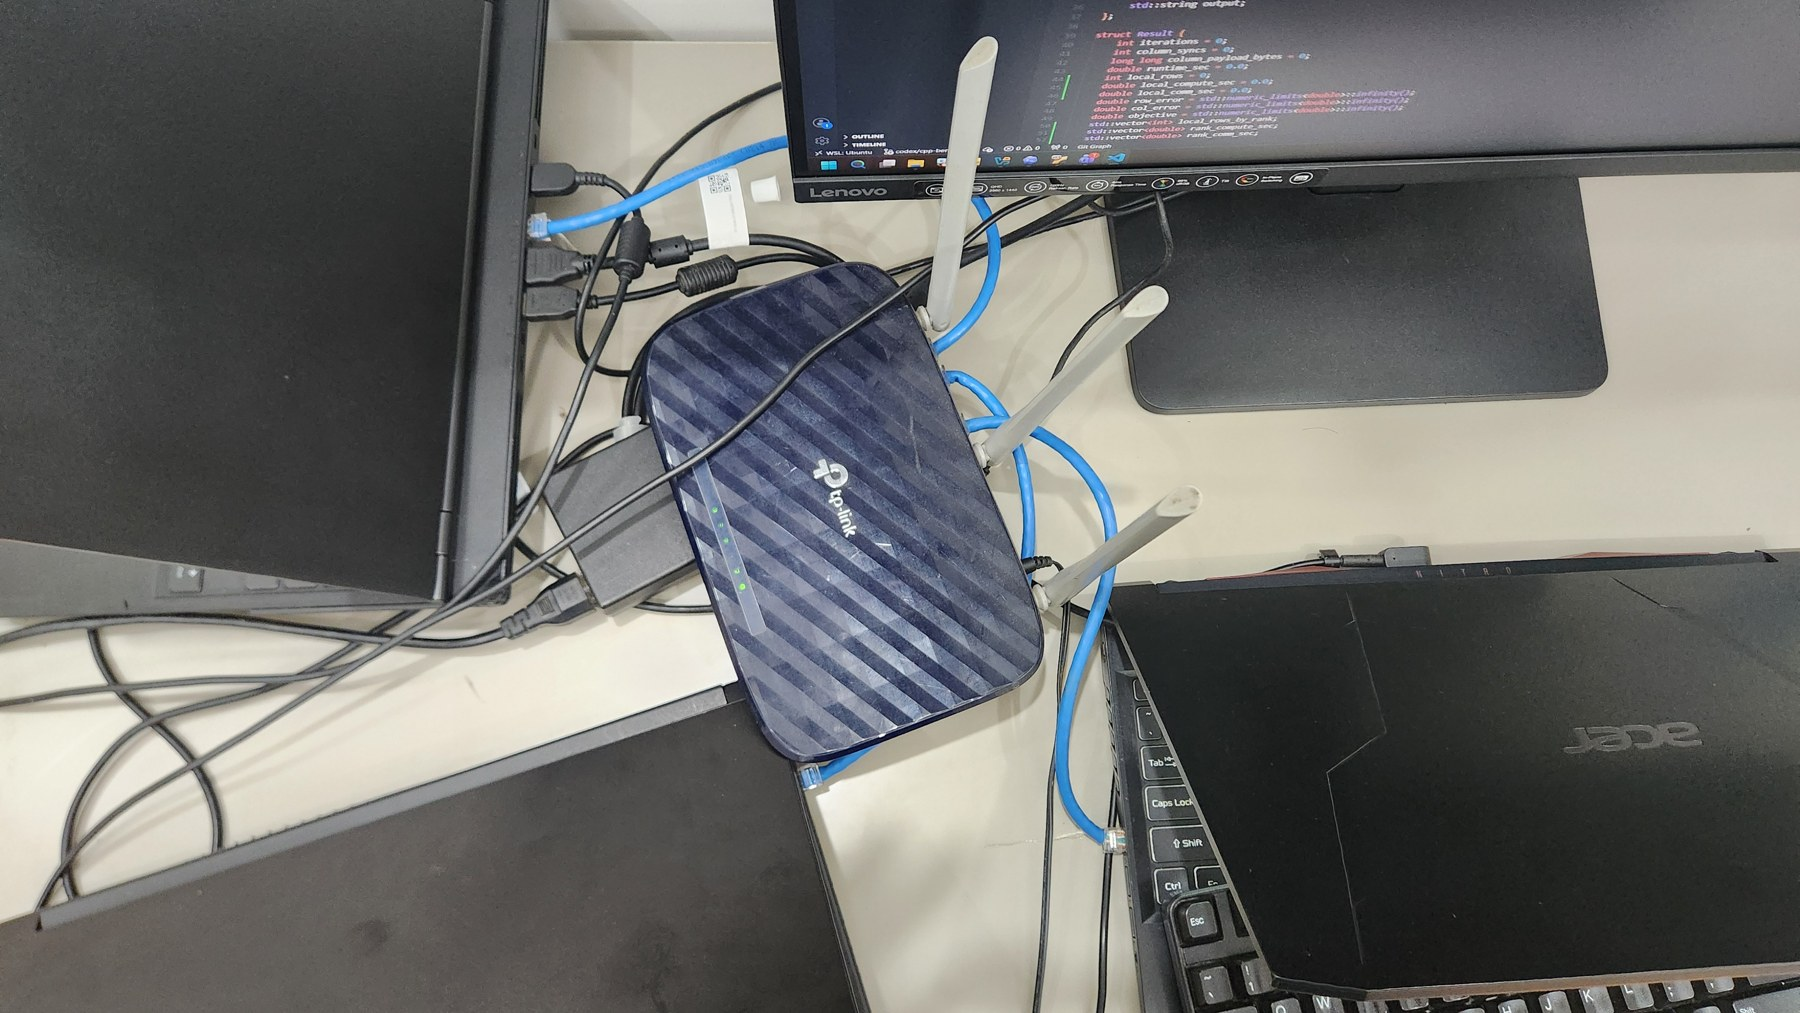
\includegraphics[height=2.6cm]{router_cluster_photo.jpg}
\end{column}
\end{columns}
\end{frame}

\section{Experiments}
\subsection{Benchmark plan}

\begin{frame}{Benchmark Plan}
\begin{enumerate}
  \item \textbf{Input-size calibration}: $N=2000..12000$, fixed 50 iterations
  \item \textbf{Long workload}: $N=8000$, increase iterations to reach 2--3 minutes
  \item \textbf{Process sweep}: vary MPI processes at fixed $N=8000$
  \item \textbf{$2N$ speedup}: run $N=16000$ with \texttt{np=1,2,4,8}
  \item \textbf{Network comparison}: router/Ethernet, Wi-Fi, phone hotspot
  \item \textbf{Dynamic scheduling}: contiguous, weighted chunks, runtime queue
\end{enumerate}
\end{frame}

\subsection{Implementation comparison}

\begin{frame}{Python Prototype vs C++ Implementation}
\begin{columns}[T]
\begin{column}{0.58\linewidth}
\centering
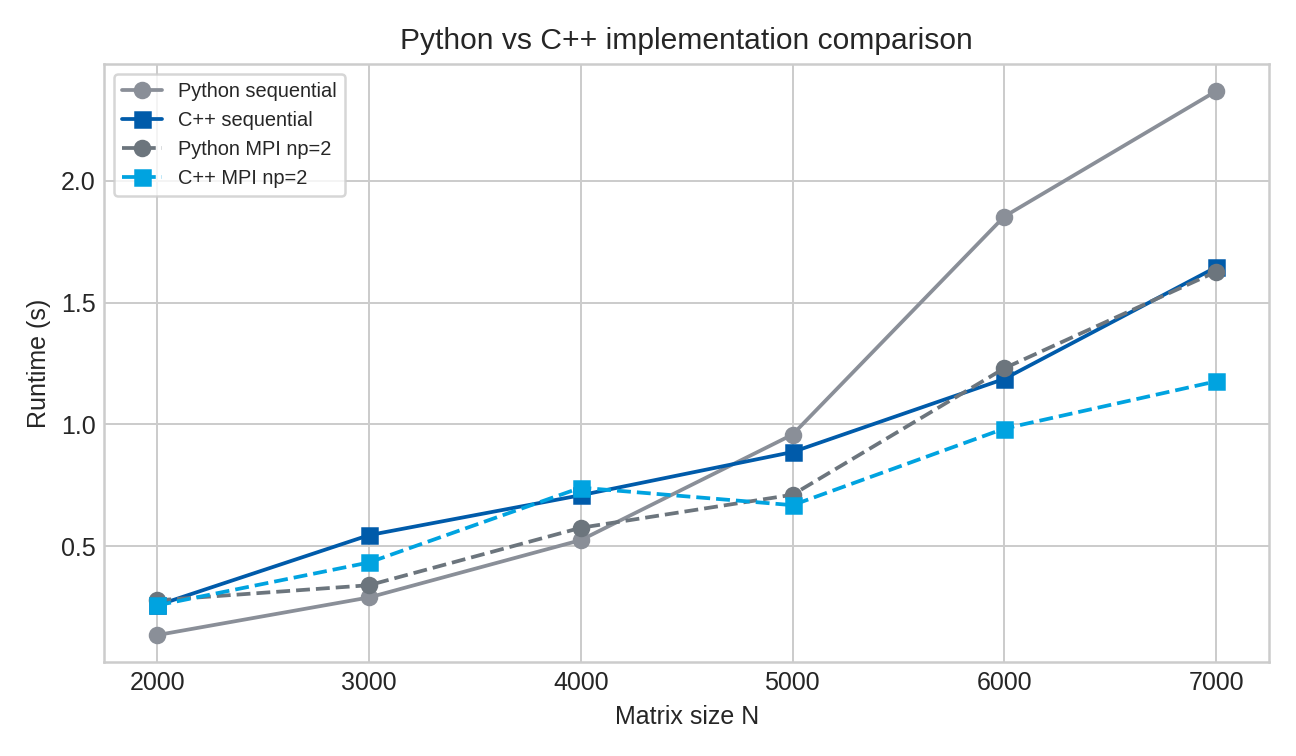
\includegraphics[width=\linewidth]{python_vs_cpp.png}
\end{column}
\begin{column}{0.38\linewidth}
\small
\textbf{Why this slide matters}
\begin{itemize}
  \item The first MVP was written in Python/mpi4py for correctness.
  \item The final submission path is C++/MPI to satisfy the course requirement.
  \item C++ becomes more attractive as the benchmark grows and avoids Python runtime overhead.
\end{itemize}
\vspace{0.15cm}
\textbf{Dataset}: two-node benchmark, 3-run averages, sizes 2000--7000.
\end{column}
\end{columns}
\end{frame}

\section{Results}
\subsection{Router and Wi-Fi}

\begin{frame}{Input-Size Sweep: Router vs Wi-Fi}
\begin{columns}
\begin{column}{0.50\linewidth}
\centering
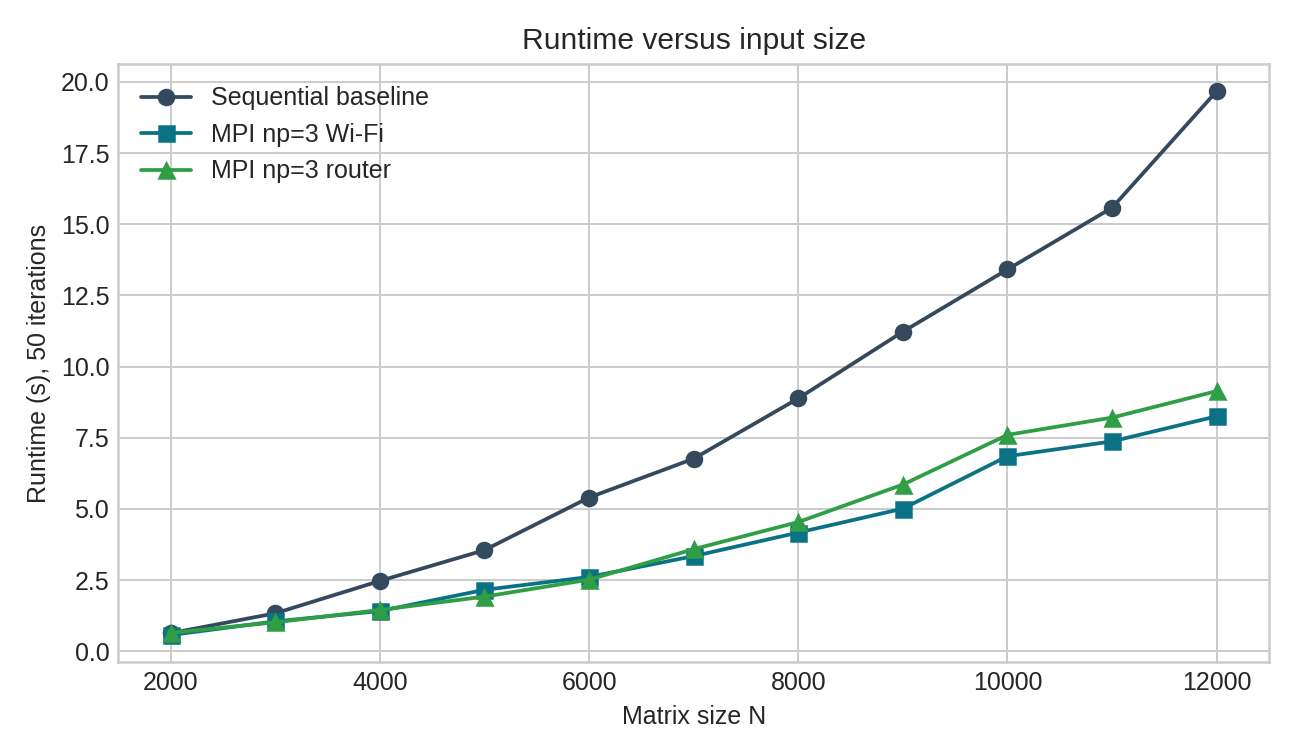
\includegraphics[width=\linewidth]{runtime_vs_size.png}
\end{column}
\begin{column}{0.50\linewidth}
\centering
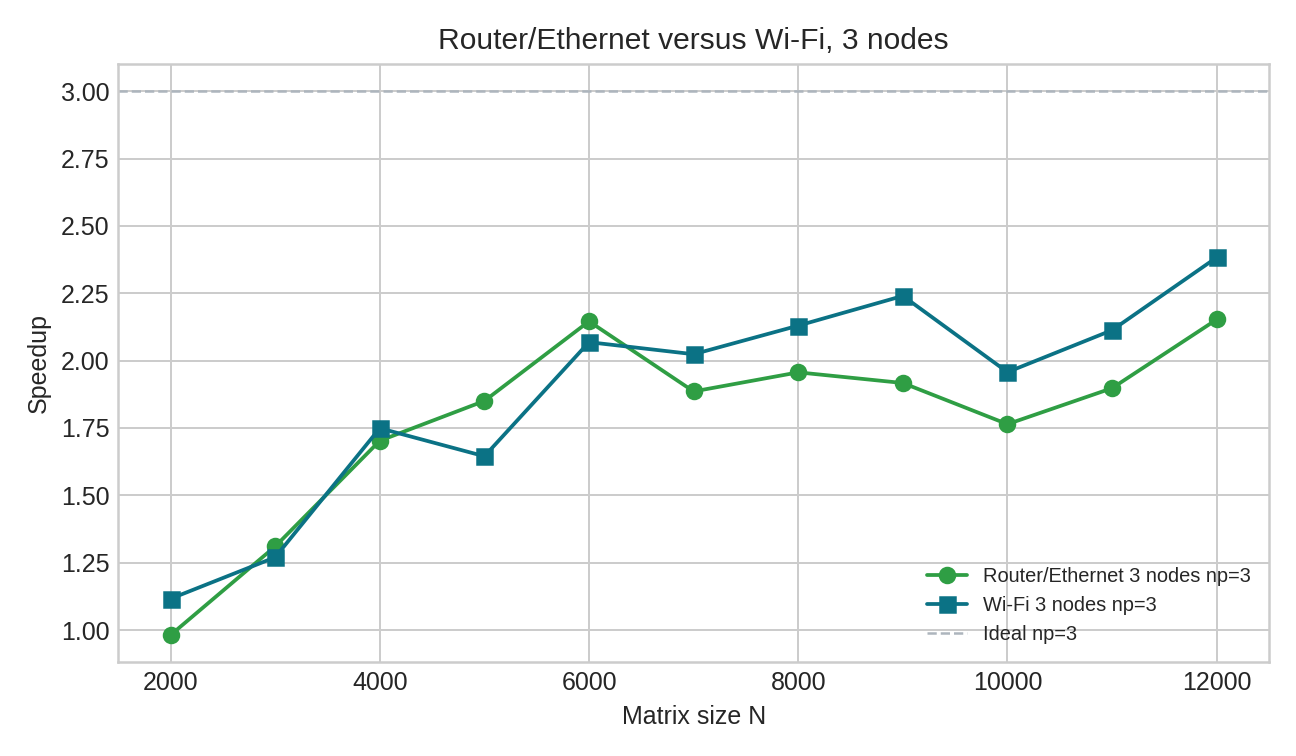
\includegraphics[width=\linewidth]{router_vs_wifi3_speedup.png}
\end{column}
\end{columns}
\vspace{0.15cm}
\small
\begin{itemize}
  \item MPI becomes useful when $N$ is large enough.
  \item At $N=12000$, Wi-Fi three-node run reaches $2.383\times$ speedup.
  \item Best observed router three-node point: $2.8859\times$ speedup, 0.962 efficiency.
\end{itemize}
\end{frame}

\subsection{Scaling}

\begin{frame}{Process Sweep and $2N$ Speedup}
\begin{columns}
\begin{column}{0.50\linewidth}
\centering
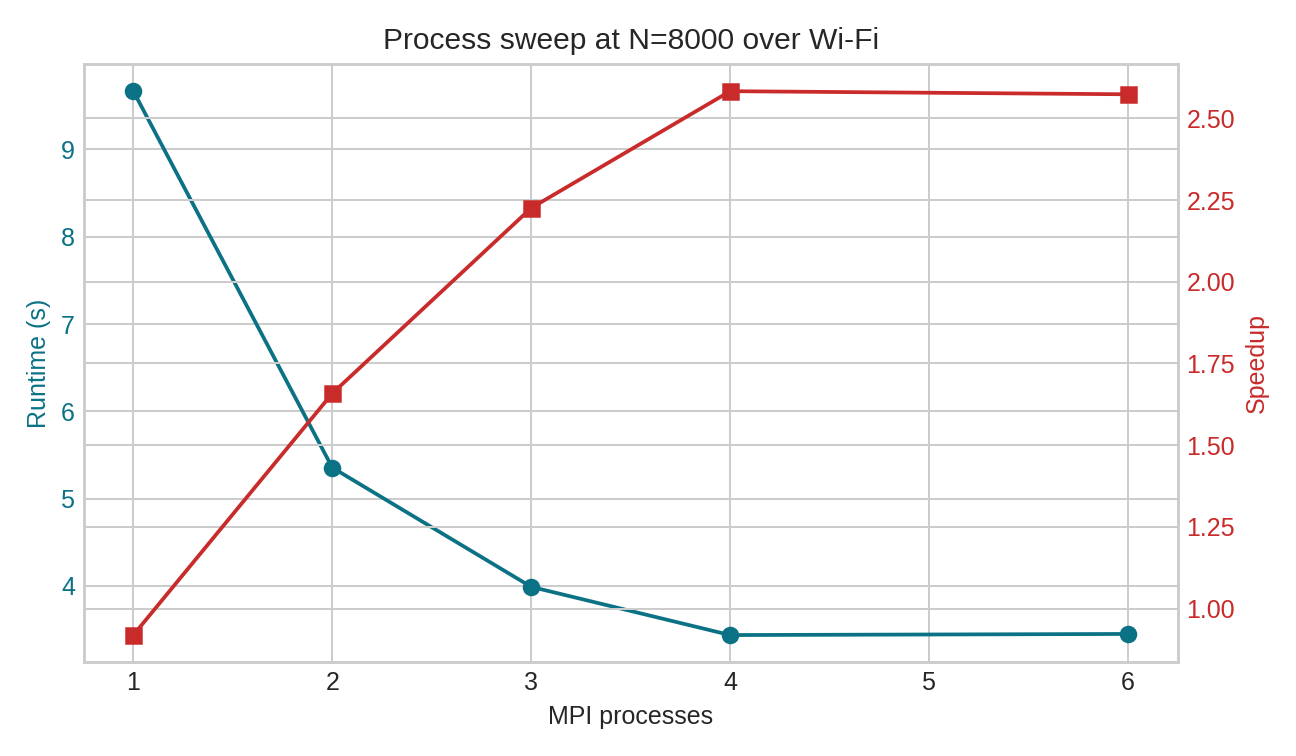
\includegraphics[width=\linewidth]{process_sweep_wifi.png}
\end{column}
\begin{column}{0.50\linewidth}
\centering
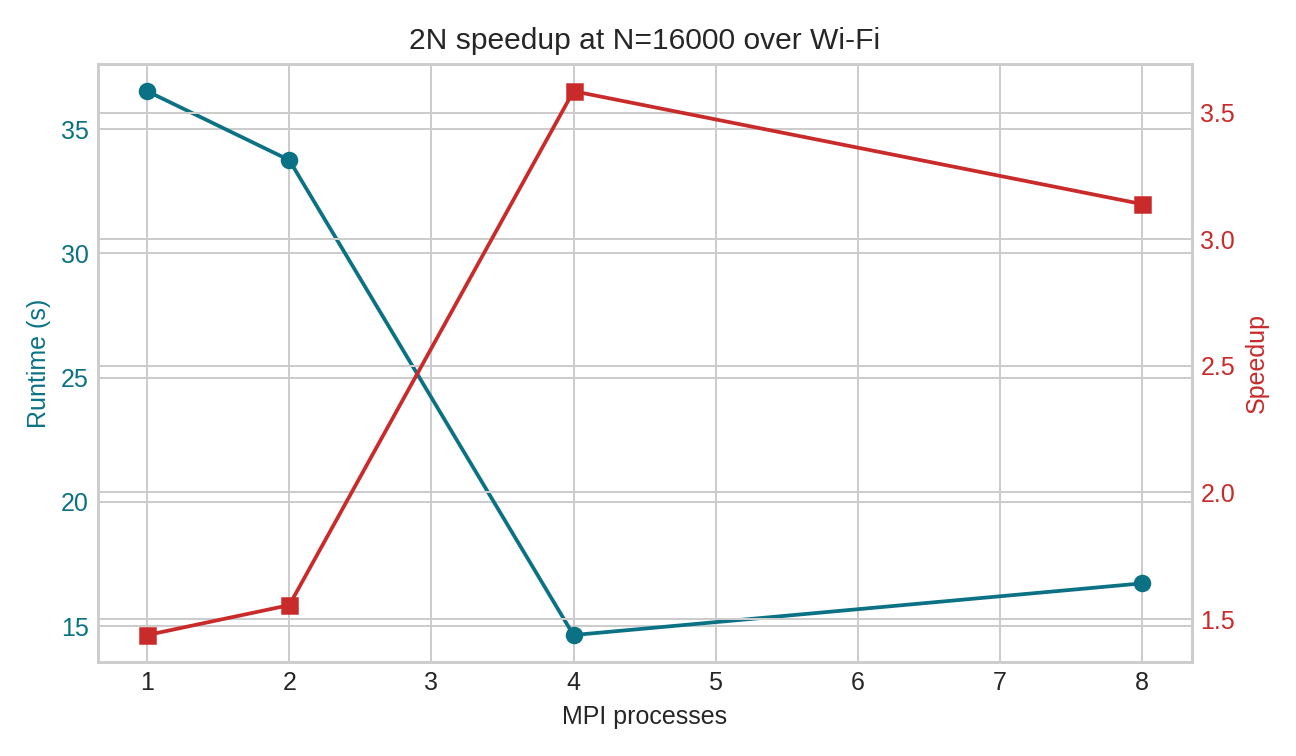
\includegraphics[width=\linewidth]{speedup_2n_wifi.png}
\end{column}
\end{columns}
\vspace{0.15cm}
\small
\begin{itemize}
  \item At $N=8000$, \texttt{np=4} is better than \texttt{np=6}.
  \item At $N=16000$, \texttt{np=4} reaches $3.585\times$ speedup.
  \item \texttt{np=8} is slower than \texttt{np=4}: communication dominates.
\end{itemize}
\end{frame}

\subsection{Calibration and load balance}

\begin{frame}{Calibration and Load Balance}
\begin{columns}
\begin{column}{0.50\linewidth}
\centering
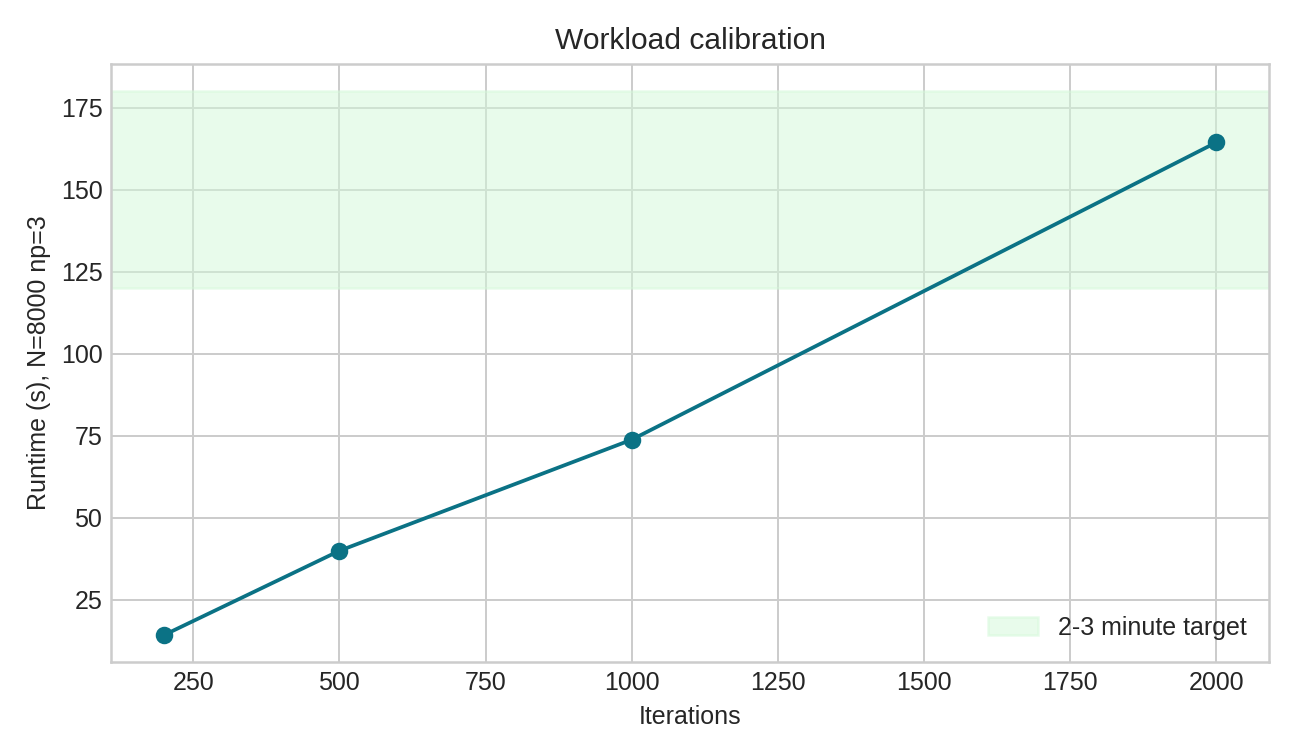
\includegraphics[width=\linewidth]{workload_calibration.png}
\end{column}
\begin{column}{0.50\linewidth}
\centering
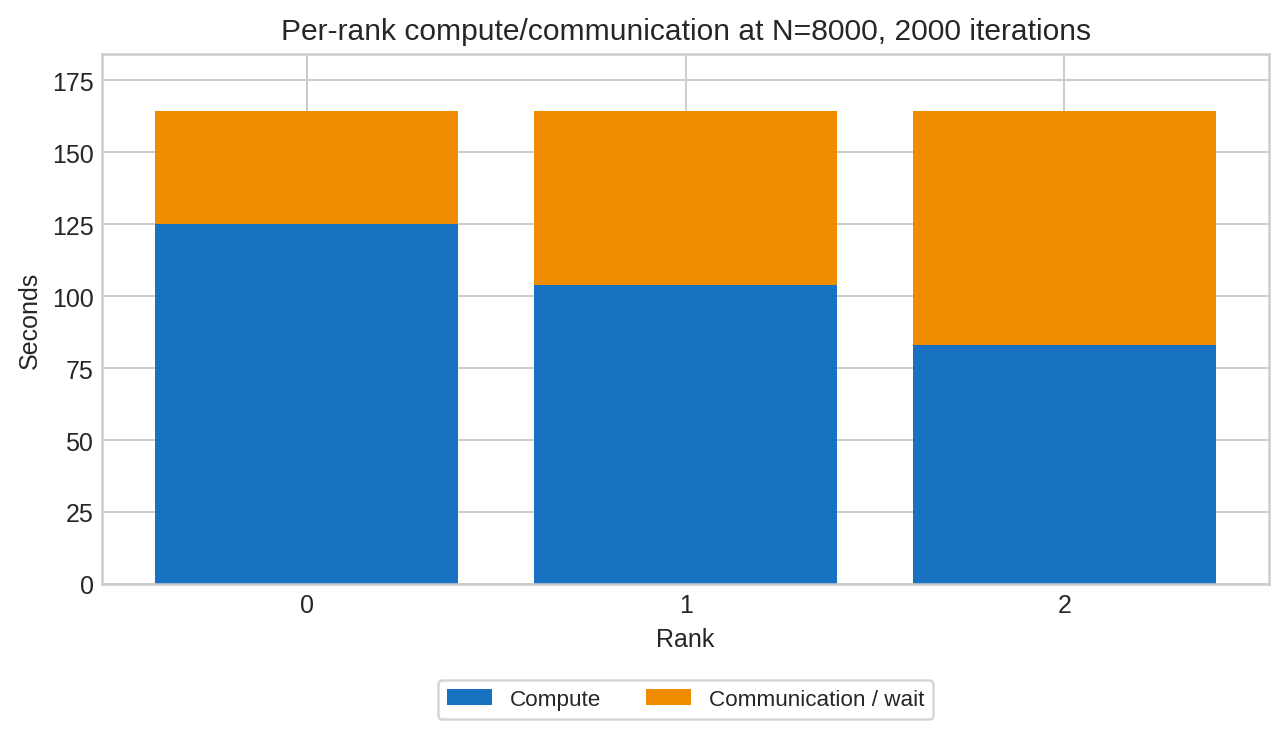
\includegraphics[width=\linewidth]{load_balance_stacked.png}
\end{column}
\end{columns}
\vspace{0.15cm}
\small
\begin{itemize}
  \item $N=8000$, 2000 iterations gives 164.394 s: within the 2--3 minute target.
  \item Total rank times are balanced, but compute/communication split reveals node heterogeneity.
\end{itemize}
\end{frame}

\subsection{Network variants}

\begin{frame}{Network and Communication Experiments}
\begin{columns}
\begin{column}{0.50\linewidth}
\centering
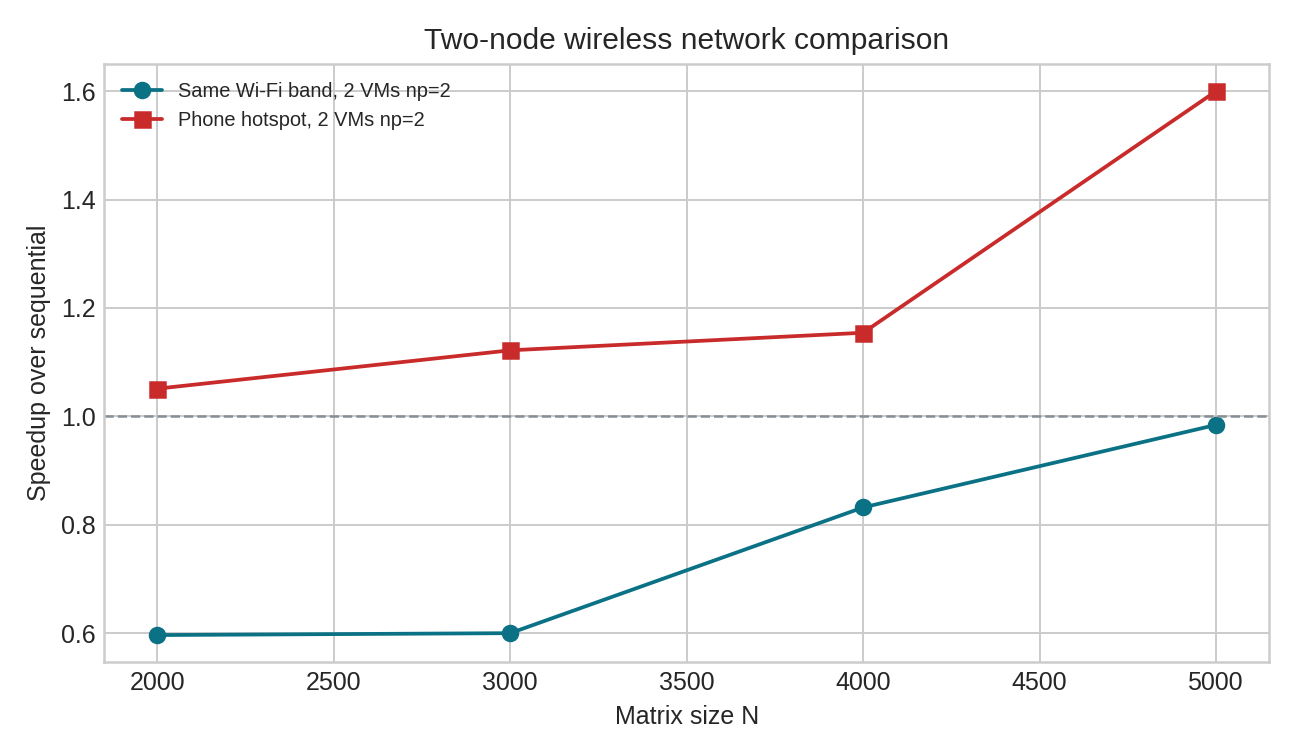
\includegraphics[width=\linewidth]{network_2node_comparison.png}
\end{column}
\begin{column}{0.50\linewidth}
\centering
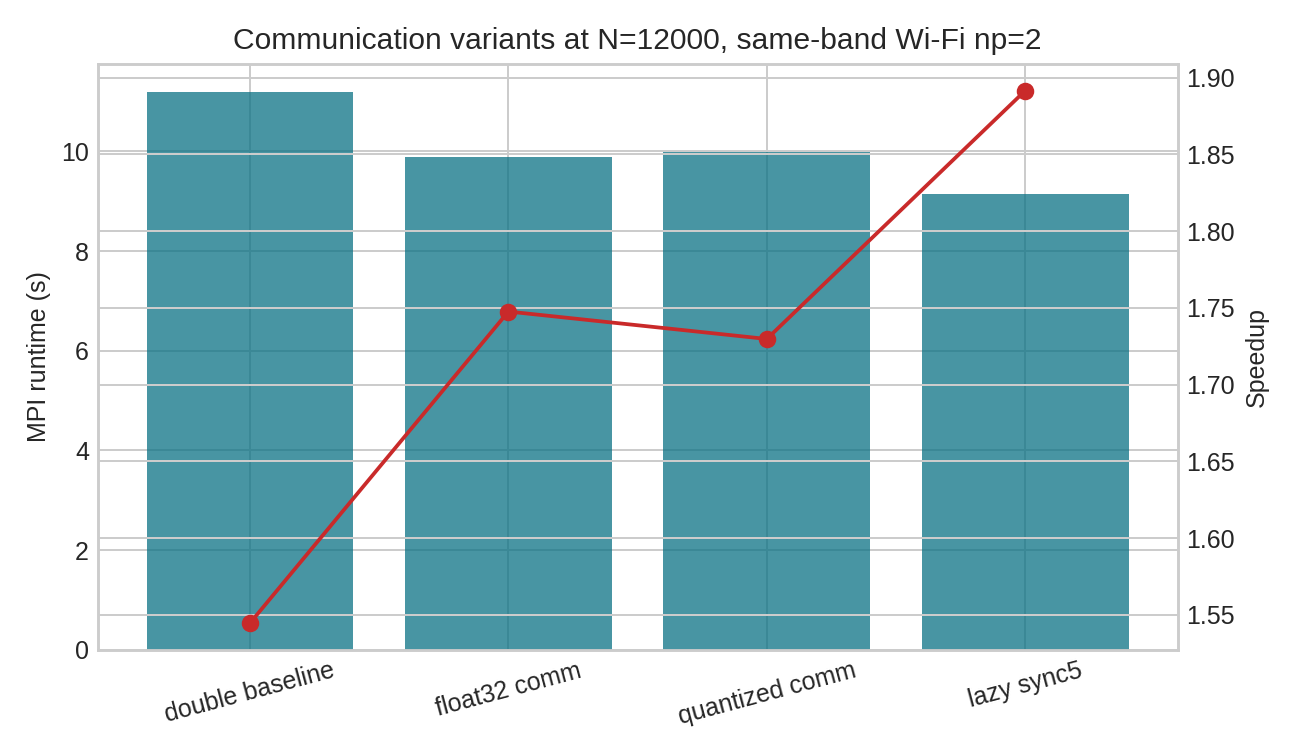
\includegraphics[width=\linewidth]{comm_variants_12000.png}
\end{column}
\end{columns}
\vspace{0.15cm}
\small
\begin{itemize}
  \item Wireless topology matters: same-band Wi-Fi and phone hotspot behave differently.
  \item Lazy sync every 5 iterations gives the best communication-variant speedup at $N=12000$.
  \item Float32 communication halves payload and is the safest compression-style optimization.
\end{itemize}
\end{frame}

\section{Dynamic Scheduling}
\subsection{Chunk-based scheduling}

\begin{frame}{Dynamic Scheduling}
\begin{columns}
\begin{column}{0.50\linewidth}
\centering
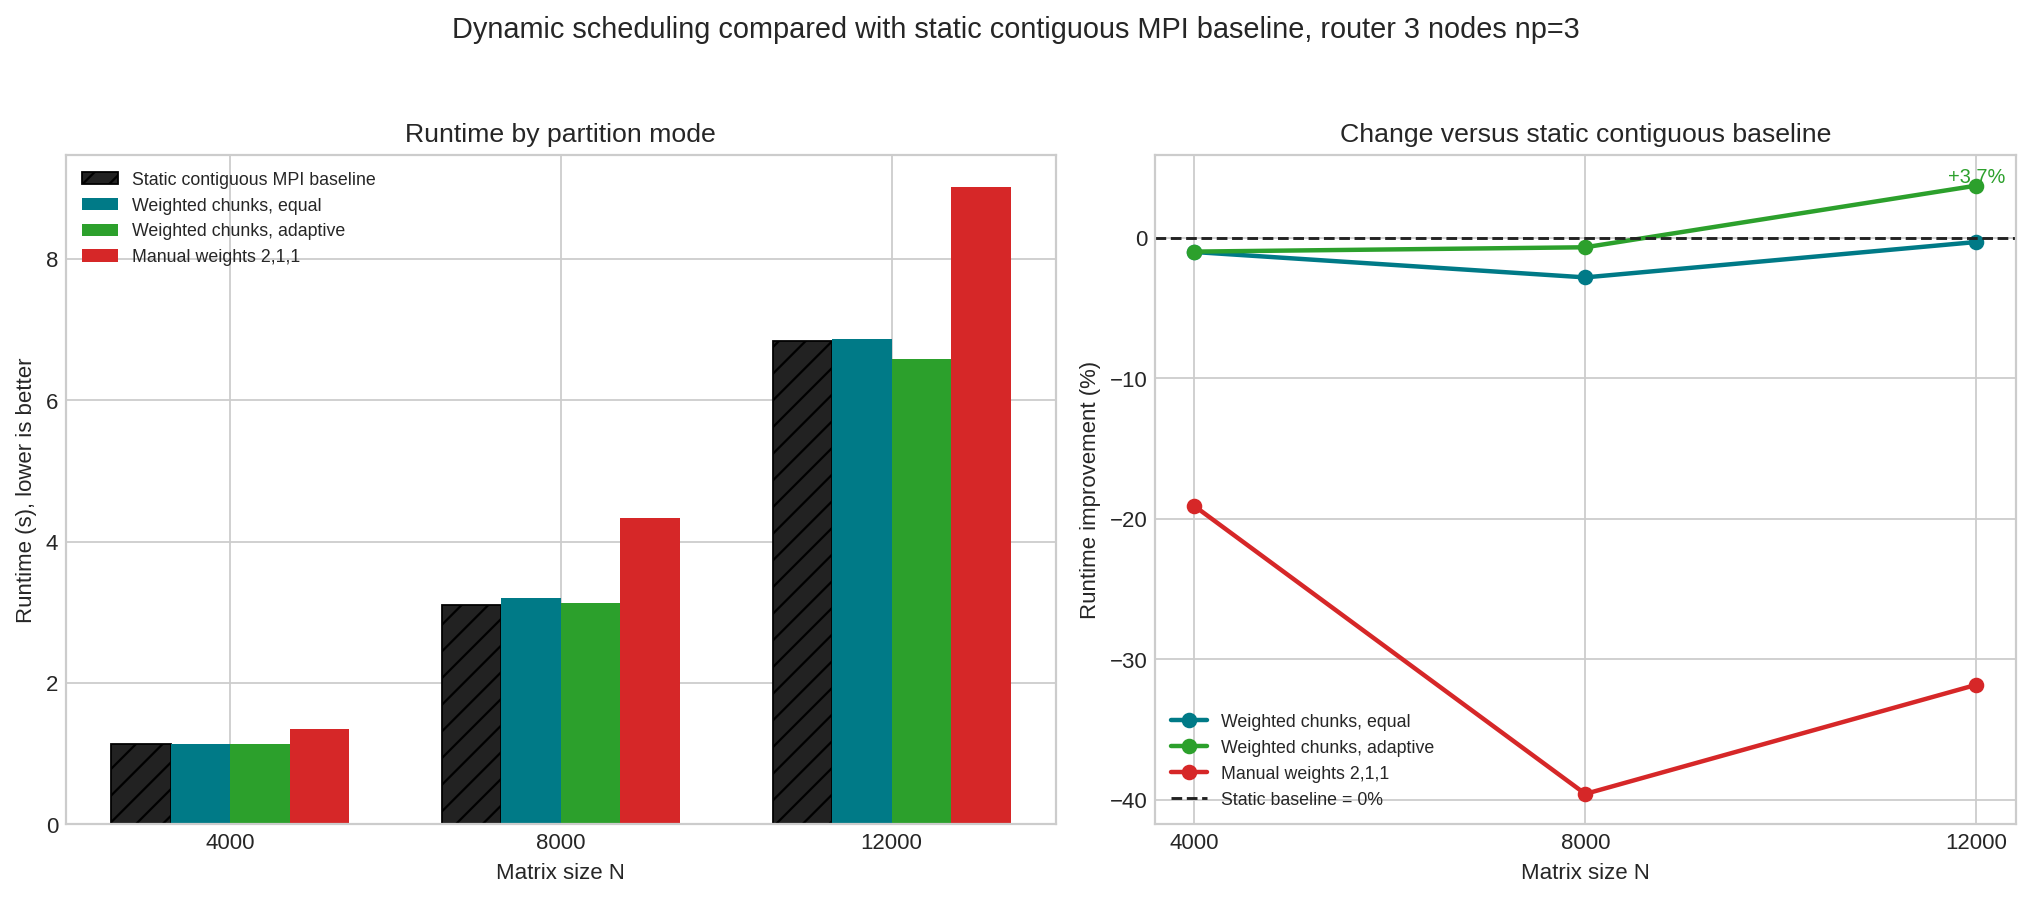
\includegraphics[width=\linewidth]{dynamic_modes_np3.png}
\end{column}
\begin{column}{0.50\linewidth}
\centering
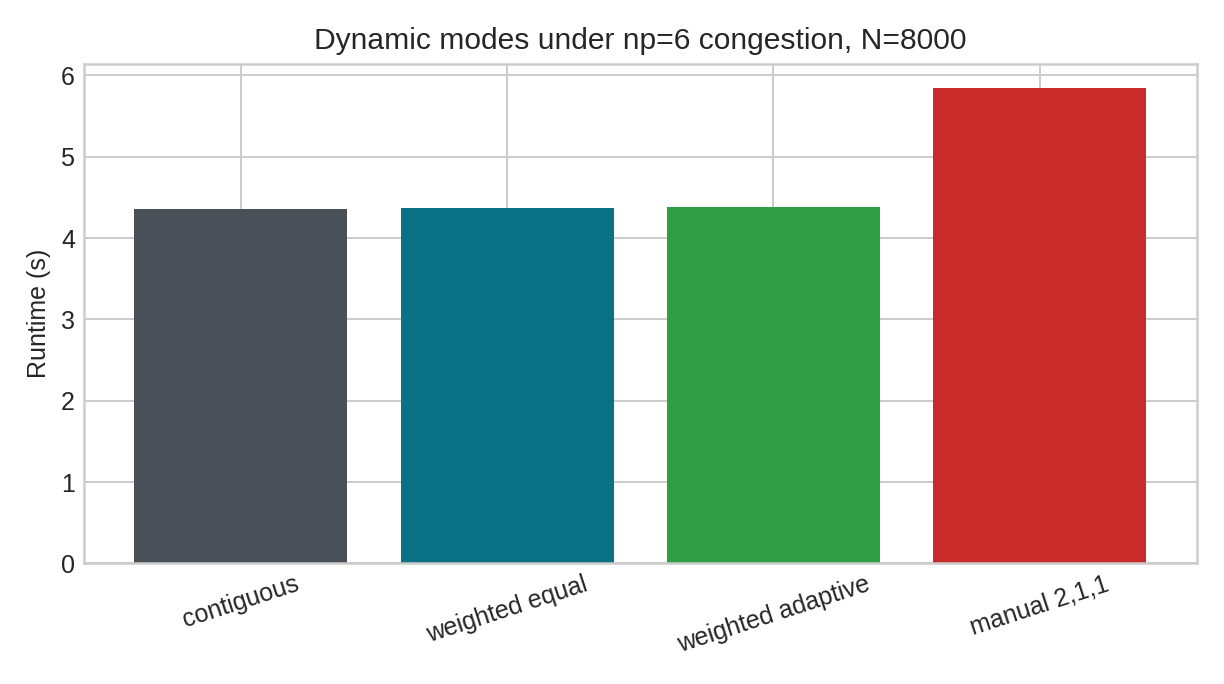
\includegraphics[width=\linewidth]{dynamic_np6_congestion.png}
\end{column}
\end{columns}
\vspace{0.15cm}
\small
\begin{itemize}
  \item Static contiguous is the MPI baseline: distributed rows, fixed ownership.
  \item Adaptive weighted chunks improve large $N=12000$ by about 3.7\% over that baseline.
  \item Manual weights can hurt if the assumed machine speeds are wrong.
  \item Runtime queue is useful for demonstration but too slow for performance.
\end{itemize}
\end{frame}

\section{Conclusion}
\subsection{Takeaways}

\begin{frame}{Conclusions}
\begin{itemize}
  \item The C++/MPI Sinkhorn solver satisfies the project requirements and runs on a real physical-machine VM cluster.
  \item Row-wise data decomposition gives clear speedup for sufficiently large dense workloads.
  \item Main bottleneck: one length-$N$ \texttt{MPI\_Allreduce} per iteration.
  \item Best stable demo recommendation:
  \begin{itemize}
    \item Router/Ethernet three-machine setup
    \item $N=8000$, 2000 iterations for a 2--3 minute workload
  \end{itemize}
  \item Dynamic weighted scheduling is a promising extension, but static contiguous partitioning remains the reliable baseline.
\end{itemize}
\end{frame}

\appendix
\section{Backup}
\subsection{Raw results}

\begin{frame}{Backup: Key Raw Result Locations}
\small
\begin{itemize}
  \item \texttt{results/bench\_cpp\_router3\_25\_26\_75\_fixed50\_reps4}
  \item \texttt{results/bench\_cpp\_router3\_report\_suite\_safe}
  \item \texttt{results/bench\_cpp\_wifi3\_25\_26\_190\_report\_suite}
  \item \texttt{results/bench\_cpp\_wifi3\_25\_26\_190\_supplemental}
  \item \texttt{results/bench\_cpp\_router3\_dynamic\_fixed50\_reps4}
  \item \texttt{results/bench\_cpp\_vm2\_sameband\_variants\_fixed50}
\end{itemize}
\end{frame}

\end{document}
